\documentclass[journal,onecolumn,twoside]{IEEEtran}


\usepackage[utf8]{inputenc}
\usepackage{graphicx}
\usepackage[justification=centering]{caption}


% *** GRAPHICS RELATED PACKAGES ***
%
\ifCLASSINFOpdf
  % \usepackage[pdftex]{graphicx}
  % declare the path(s) where your graphic files are
  % \graphicspath{{../pdf/}{../jpeg/}}
  % and their extensions so you won't have to specify these with
  % every instance of \includegraphics
  % \DeclareGraphicsExtensions{.pdf,.jpeg,.png}
\else
  % or other class option (dvipsone, dvipdf, if not using dvips). graphicx
  % will default to the driver specified in the system graphics.cfg if no
  % driver is specified.
  % \usepackage[dvips]{graphicx}
  % declare the path(s) where your graphic files are
  % \graphicspath{{../eps/}}
  % and their extensions so you won't have to specify these with
  % every instance of \includegraphics
  % \DeclareGraphicsExtensions{.eps}
\fi
% graphicx was written by David Carlisle and Sebastian Rahtz. It is
% required if you want graphics, photos, etc. graphicx.sty is already
% installed on most LaTeX systems. The latest version and documentation
% can be obtained at: 
% http://www.ctan.org/pkg/graphicx
% Another good source of documentation is "Using Imported Graphics in
% LaTeX2e" by Keith Reckdahl which can be found at:
% http://www.ctan.org/pkg/epslatex
%
% latex, and pdflatex in dvi mode, support graphics in encapsulated
% postscript (.eps) format. pdflatex in pdf mode supports graphics
% in .pdf, .jpeg, .png and .mps (metapost) formats. Users should ensure
% that all non-photo figures use a vector format (.eps, .pdf, .mps) and
% not a bitmapped formats (.jpeg, .png). The IEEE frowns on bitmapped formats
% which can result in "jaggedy"/blurry rendering of lines and letters as
% well as large increases in file sizes.
%
% You can find documentation about the pdfTeX application at:
% http://www.tug.org/applications/pdftex



% *** Do not adjust lengths that control margins, column widths, etc. ***
% *** Do not use packages that alter fonts (such as pslatex).         ***
% There should be no need to do such things with IEEEtran.cls V1.6 and later.
% (Unless specifically asked to do so by the journal or conference you plan
% to submit to, of course. )


% correct bad hyphenation here
\hyphenation{op-tical net-works semi-conduc-tor}


\begin{document}
%
% paper title
% Titles are generally capitalized except for words such as a, an, and, as,
% at, but, by, for, in, nor, of, on, or, the, to and up, which are usually
% not capitalized unless they are the first or last word of the title.
% Linebreaks \\ can be used within to get better formatting as desired.
% Do not put math or special symbols in the title.
\title{Evaluating Lévy Flight Parameters for
Random Searches in a 2D Space}
%
%
% author names and IEEE memberships
% note positions of commas and nonbreaking spaces ( ~ ) LaTeX will not break
% a structure at a ~ so this keeps an author's name from being broken across
% two lines.
% use \thanks{} to gain access to the first footnote area
% a separate \thanks must be used for each paragraph as LaTeX2e's \thanks
% was not built to handle multiple paragraphs
%

\author{Mario~González, %~\IEEEmembership{Member,~IEEE,}
        John~Doe, %~\IEEEmembership{Fellow,~OSA,}
        and~Jane~Doe. %,~\IEEEmembership{Life~Fellow,~IEEE}% <-this % stops a space
\thanks{Director: David Dominguez.}% <-this % stops a space
%\thanks{J. Doe and J. Doe are with Anonymous University.}% <-this % stops a space
\thanks{Manuscript elaborated April 19, 2005; revised August 26, 2015.}}



% The paper headers
\markboth{Nombre de los tesistas}%
{Titulo de la tesis}




% make the title area
\maketitle

% As a general rule, do not put math, special symbols or citations
% in the abstract or keywords.
\begin{abstract}
It is experimentally known that the 
flight lengths of random searches by 
foragers such as honey bees statistically 
belong to a power law distribution.
Optimality of such random searches has been 
a topic of extensive research because 
knowing their optimal parameters may help applied sciences. 
Viswanathan have shown the inverse-square power law 
to be the optimal law for such random searches. 
%
This thesis explores the capability of the model 
presented in such that it can be applied to 
Unmanned Autonomous Vehicles
(UAVs). The thesis also identifies the minimum 
flight length, $l_{min}$, as an important factor 
that needs to be controlled based on the UAV’s 
sensor range.
We present a theoretical lmin as an explicit 
function of the sensor range, $rv$,
and an estimated target density, $\rho$.
\end{abstract}

% Note that keywords are not normally used for peerreview papers.
\begin{IEEEkeywords}
Levy distribution, Random walks, parameter optimization.
\end{IEEEkeywords}



\IEEEpeerreviewmaketitle

\tableofcontents

\section{Introduction}


\IEEEPARstart{R}{ecent} 
observation made about foraging animals is that foragers when in
no or limited prior knowledge of food show searching patterns that have
special characteristics. The patterns are different from what can be seen in
Brownian motion, the random walk by particles diffusing in a liquid. Foragers
sometimes take long paths in just one direction. This strategy is found to
be the key to the foragers’ success in finding food rapidly in an unknown
environment \cite{reynolds2007honeybees}.

It is shown experimentally that these foragers often take an optimal random searching strategy \cite{reynolds2007honeybees}. 
The experimental method in \cite{reynolds2007honeybees} includes tracking
honeybees using harmonic radar tracking, 
and fitting the found flight lengths
to a probability distribution. 
The flight lengths fit in to a Levy like characteristic with the optimal parameters proposed earlier and independently
in \cite{reynolds2007honeybees, viswanathan1999optimizing}. Viswanathan et al. analytically show that the optimal strategy for
random searches is an inverse-square power law distribution for any general
case based on \textbf{an idealized foraging model.} Their analytical model closely
represents the forager-food relationship. 

Next section \ref{model} is defined as follows.

\section{Model}
\label{model}

\subsection{Foraging model}

The discrete case, in Eq. (\ref{eq:C}), $C$, is defined as:
\begin{equation}
    C = \left( \sum_{n=0}^{\infty} (n \times l_{min})^{-\mu} \right)^{-\mu}.
    \label{eq:C}
\end{equation}

\subsection{Probability distribution}

Power-law distributions have a wide range of appearances in different fields.
In a target searching context, flight lengths, $l$, are said to have the power-law
distribution when all these lengths are drawn from a probability distribution of the form
\begin{equation}
  p(l) \approx l^{-\mu},   
\end{equation}
where $\mu$ is the scaling parameter.


In Fig. \ref{fig:c1} is depicted

\begin{figure}[t]
\centering
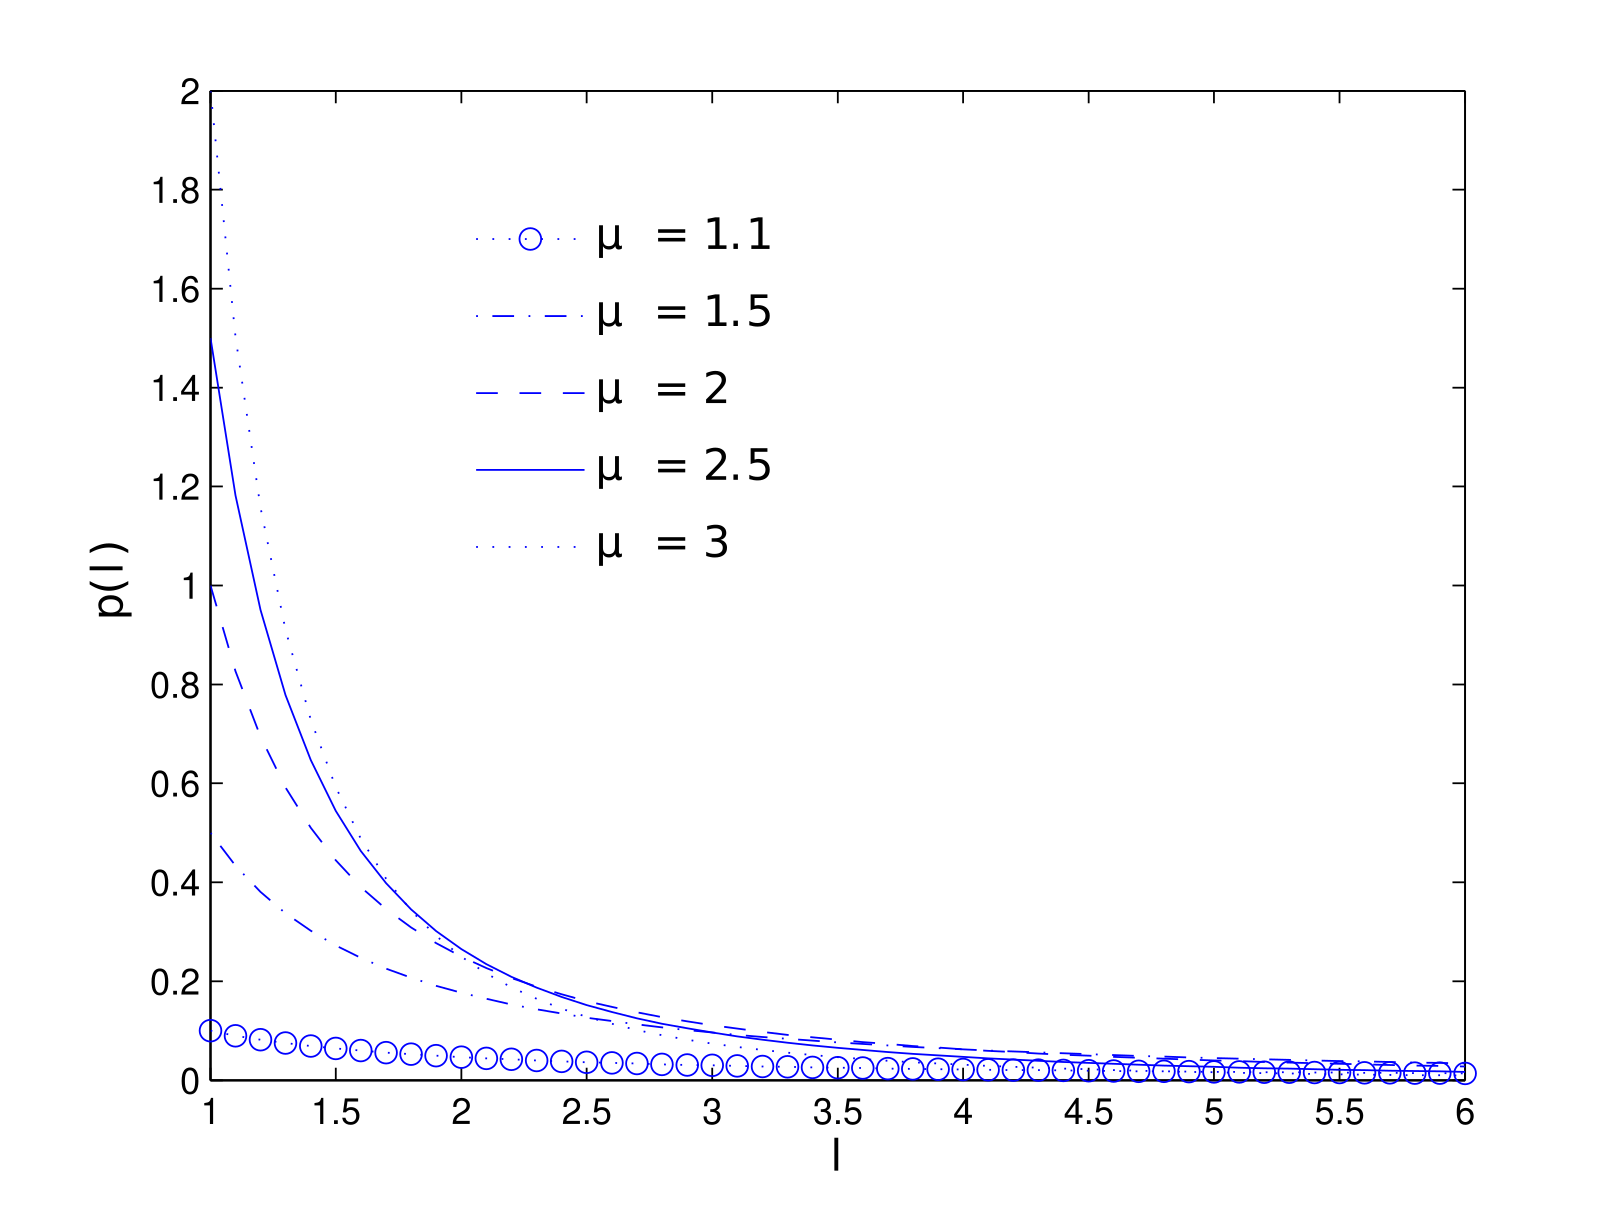
\includegraphics[scale=1]{g12.png}
\caption{Example of optimization.}
\label{fig:c1}
\end{figure}


\section{Results}
\label{results}

\begin{enumerate}
    \item First result
    \item Second results
    \begin{enumerate}
        \item Result a of second result.
    \end{enumerate}
\end{enumerate}

\begin{itemize}
    \item First result
    \item Second results
    \begin{itemize}
        \item Result a of second result.
    \end{itemize}
\end{itemize}

\subsection{Add a table}

\begin{center}
\begin{tabular}{ |l|c|r| }
 \hline
 \textbf{Col1: Left} & Col2: Center & Col3: Right \\ \hline
 cell4 & cell5 & cell6 \\ \hline
 cell7 & cell8 & cell9 \\ 
 \hline
\end{tabular}
\end{center}



\section{Conclusion}
The conclusion goes here.



\appendices
\section{Proof of the First Zonklar Equation}
Appendix one text goes here.

% you can choose not to have a title for an appendix
% if you want by leaving the argument blank
\section{}
Appendix two text goes here.


% use section* for acknowledgment
\section*{Acknowledgment}


The authors would like to thank...


% Can use something like this to put references on a page
% by themselves when using endfloat and the captionsoff option.
\ifCLASSOPTIONcaptionsoff
  \newpage
\fi



\bibliographystyle{IEEEtran}
% argument is your BibTeX string definitions and bibliography database(s)
\bibliography{referencias.bib}


\begin{IEEEbiography}{Michael Shell}
Biography text here.
\end{IEEEbiography}

% if you will not have a photo at all:
\begin{IEEEbiographynophoto}{John Doe}
Biography text here.
\end{IEEEbiographynophoto}

% insert where needed to balance the two columns on the last page with
% biographies
%\newpage

\begin{IEEEbiographynophoto}{Jane Doe}
Biography text here.
\end{IEEEbiographynophoto}




% that's all folks
\end{document}